\documentclass[11pt]{article}
\usepackage{amsmath}
\usepackage{graphicx}
\usepackage[margin=0.5in]{geometry}

\begin{document}
\title{CS280 Homework 1}
\author{Richard Hwang}
\maketitle

\section{Perspective Projection}
\begin{enumerate}
\item
    Take two arbitrary lines lying in the same plane,
    $\vec{a_1} + \lambda\vec{d}$ and $\vec{a_2} + \lambda\vec{e}$.  We know
    the vanishing points of these two lines are $f\frac{\vec{d}}{d_z}$ and
    $f\frac{\vec{e}}{e_z}$. Furthermore, because they lie in the same plane, we
    know $\vec{d} \times \vec{e} = \vec{n}$, where $\vec{n}$ is the normal
    vector of the plane. Finally, the vanishing line of a plane is
    $xn_x + yn_y + fn_z = 0$.  Using these facts, we will show the vanishing
    point of the lines are in fact on the vanishing line of the plane.

    $$\vec{n} = \begin{pmatrix}d_ye_z - d_ze_y&d_ze_x-d_xe_z&d_xe_y-e_xd_y\end{pmatrix}$$
    Plugging the vanishing points of the lines into the vanishing line...
    $$f\frac{d_x}{d_z}(d_ye_z - d_ze_y) + f\frac{d_y}{d_z}(d_ze_x-d_xe_z)
    + f(d_xe_y-e_xd_y) = 0$$
    $$\frac{d_xd_ye_z}{d_z} - \frac{d_xd_ze_y}{d_z} + \frac{d_yd_ze_x}{d_z} -
    \frac{d_xd_ye_z}{d_z} + d_xe_y - e_xd_y= 0$$
    $$0 = 0$$

    $$f\frac{e_x}{e_z}(d_ye_z - d_ze_y) + f\frac{e_y}{e_z}(d_ze_x-d_xe_z)
    + f(d_xe_y-e_xd_y) = 0$$
    $$\frac{e_xd_ye_z}{e_z} - \frac{e_xd_ze_y}{e_z} + \frac{e_yd_ze_x}{e_z} -
    \frac{e_yd_xe_z}{e_z} + d_xe_y - e_xd_y= 0$$
    $$0 = 0$$

\item
\item
    Define $\theta$ as the angle between the observer's body and the point.

    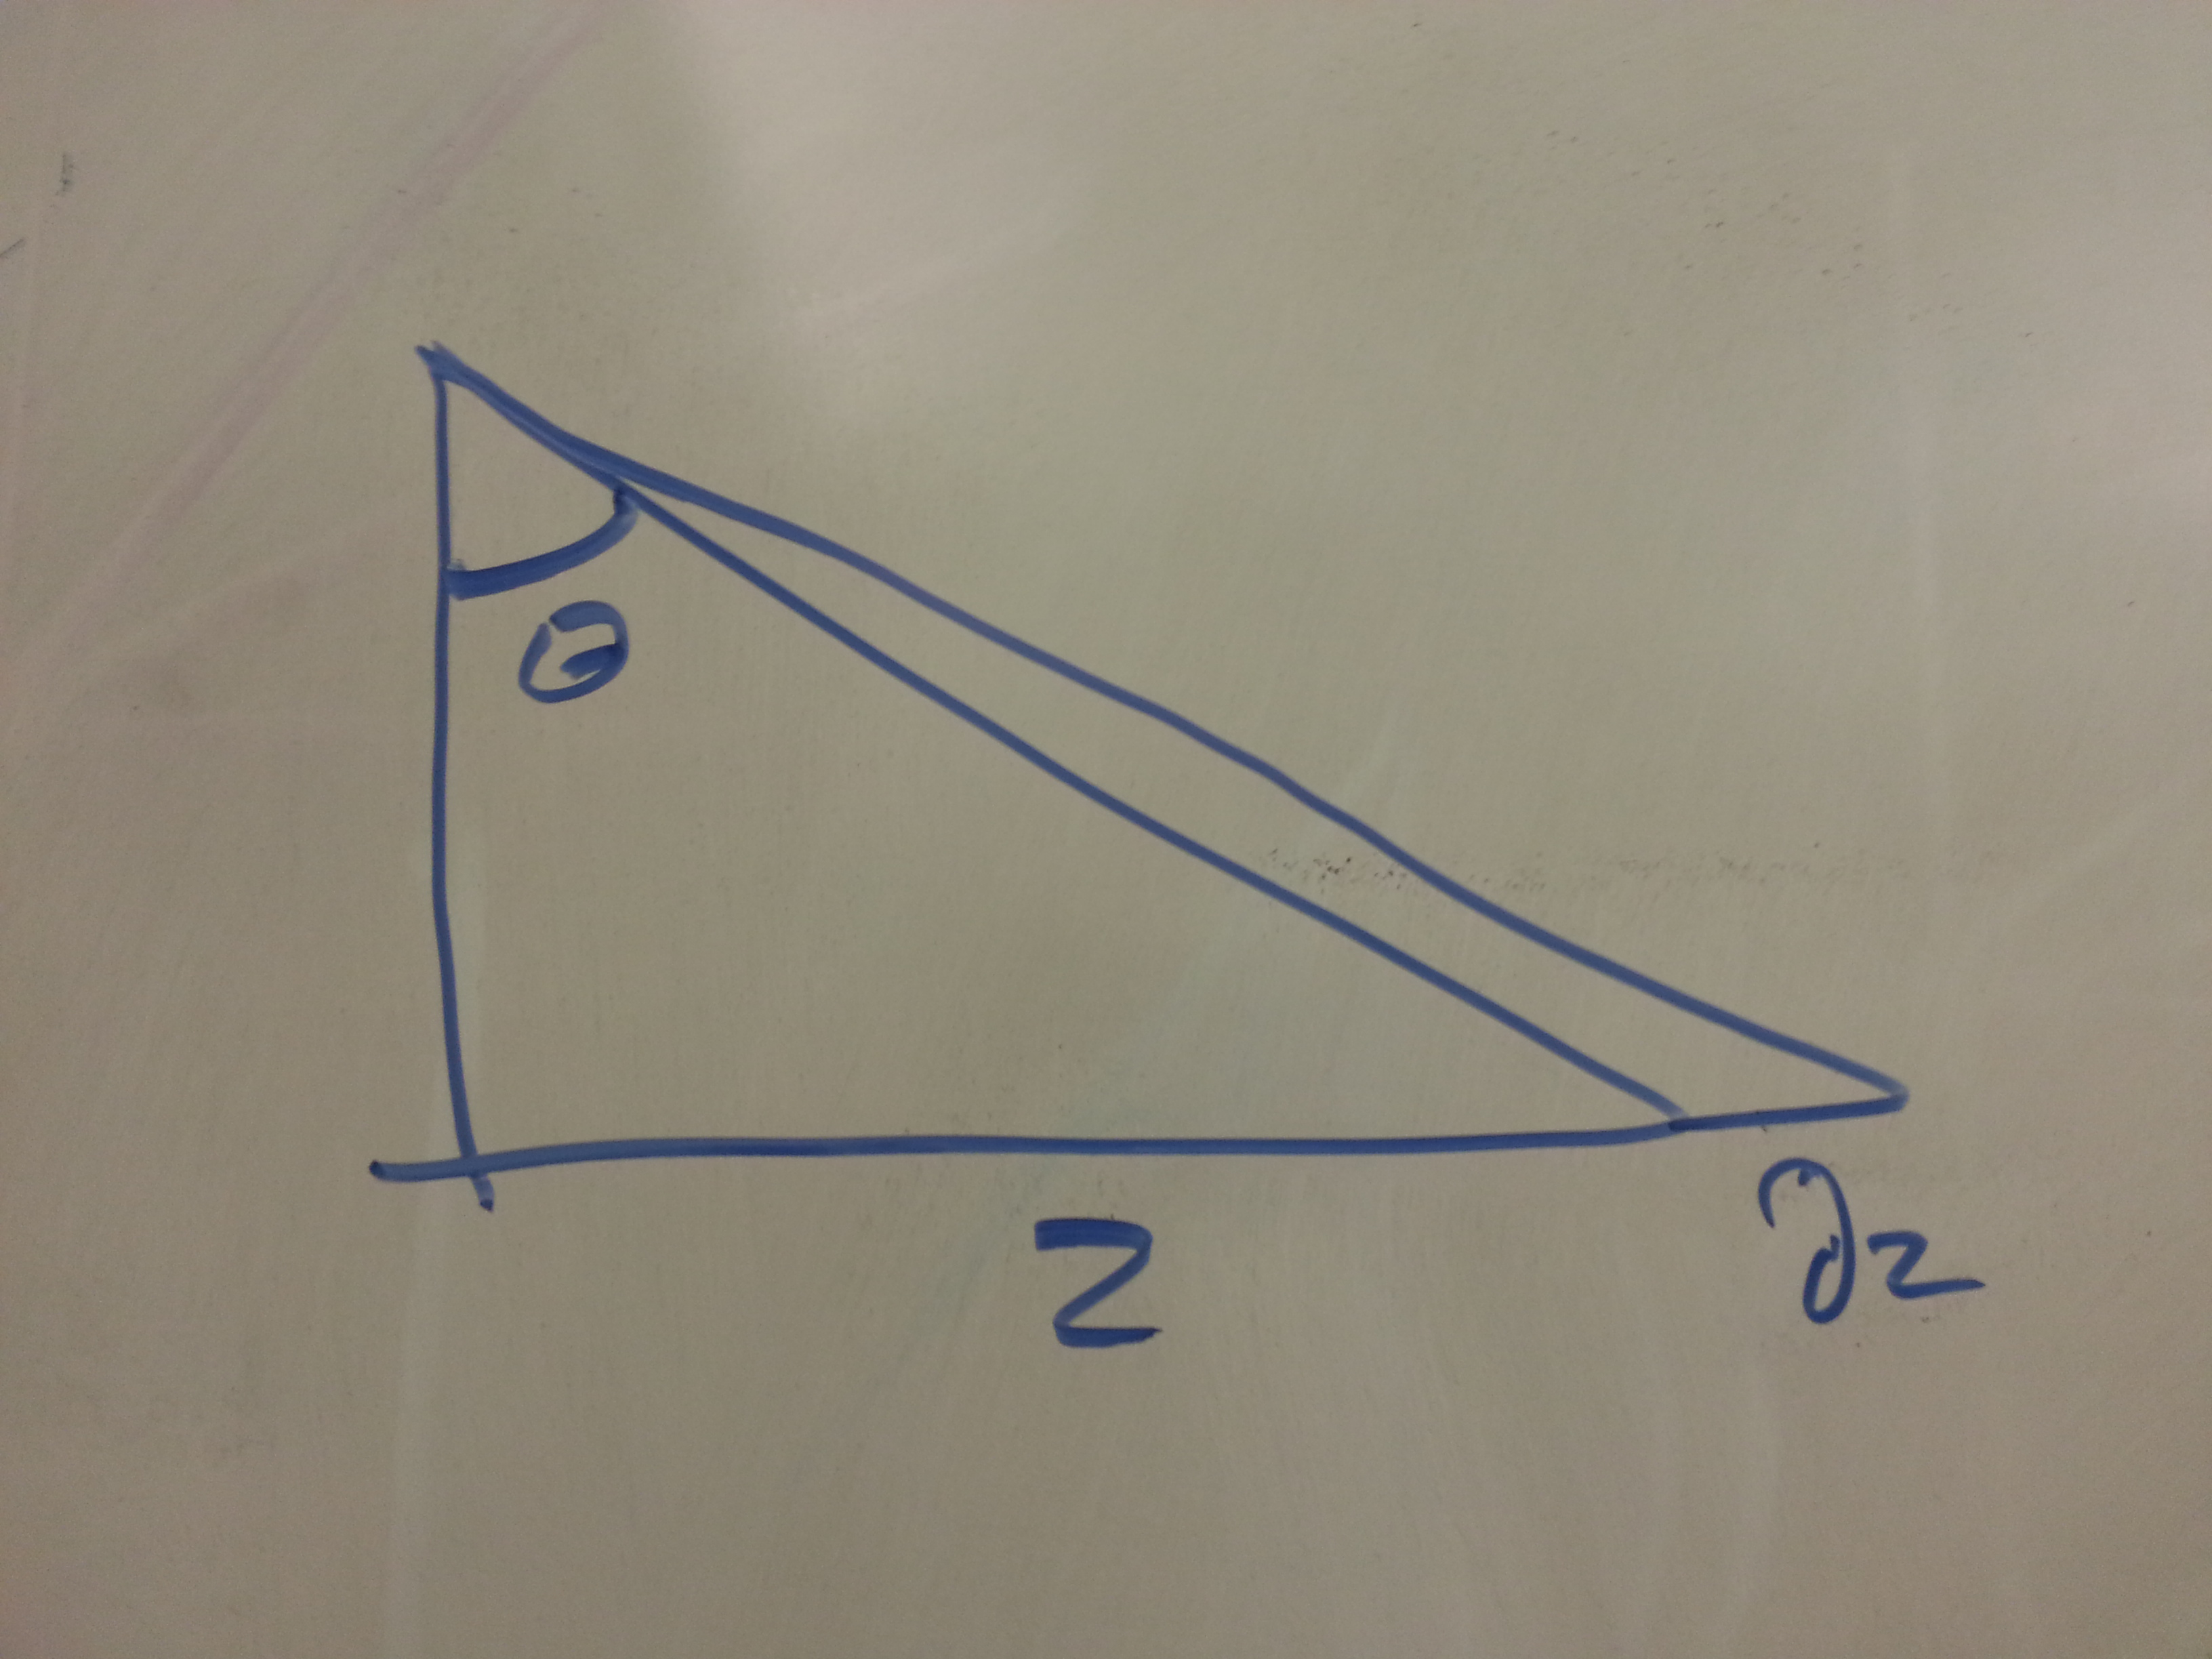
\includegraphics[width=0.5\linewidth]{./../img/delta_z.jpg}

    $$\theta = arctan(\frac{z}{h})$$
    $$tan(\theta + 1') = \frac{x + \delta z}{h}$$
    $$\delta z = h*tan(tan^{-1}(\frac{z}{h}) + 1') - z$$
\end{enumerate}
\newpage

\section{Tour into the Picture}
\begin{enumerate}
\item To estimate the 3D geometry of the room, we take advantage of the fact
    that the back plane is parallel to the image plane, and the other walls
    are perpendicular to it.  If we know the back plane along with the
    vanishing point, we know the relative camera position in the room.
    Furthermore, if we assume a focal length, we can calculate the depth of
    the room, using similar triangles.

    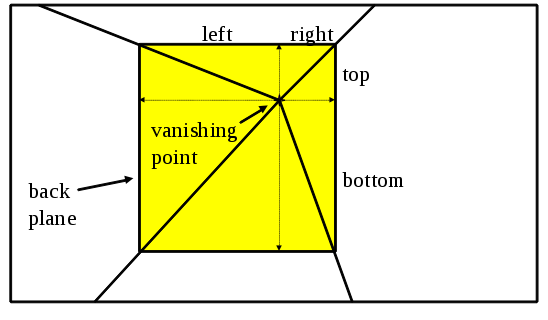
\includegraphics[width=0.5\linewidth]{./../img/3d_geometry.png}

\item To compute each of the homographies, we solve for $H$ given $s$ and $d$,
    source and destination points. A homography must map $s$ to $d$.
    $$\vec{d} = H\vec{s}$$
    
    Writing this out explicitly:
    $$\begin{pmatrix}wx'\\wy'\\w\end{pmatrix} = 
    \begin{pmatrix}a&b&c\\d&e&f\\g&h&1\end{pmatrix}
    \begin{pmatrix}x\\y\\1\end{pmatrix}$$
    $$wx'=ax + by + c$$
    $$wy'=dx + ey + f$$
    $$w=gx + hy + 1$$

    If we plug in the equation for $w$ into the first two, we get:
    $$ax + by + c - gxx' - hyx' = x'$$
    $$dx + ey + f - gxy' - hyy' = y'$$

    Given a pair of source/destination points, we get two equations.  Thus, we
    need four pairs of points to generate the eight equations we need to solve
    for the homography.  Writing those equations in matrix form, with
    $(x_i',y_i')$ as the ith destination point:
    $$\begin{pmatrix}x_1 & y_1 & 1 & 0 & 0 & 0 & -x_1x_1' & y_1x_1'\\
    0 & 0 & 0 & x_1 & y_1 & 1 & -x_1y_1' & y_1y_1'\\
    x_2 & y_2 & 1 & 0 & 0 & 0 & -x_2x_2' & y_2x_2'\\
    0 & 0 & 0 & x_2 & y_2 & 1 & -x_2y_2' & y_2y_2'\\
    ...\end{pmatrix}
    \begin{pmatrix}a\\b\\c\\d\\e\\f\\g\\h\end{pmatrix} =
    \begin{pmatrix}x_1'\\y_1'\\x_2'\\y_2'\\...\end{pmatrix}$$
    $$Ah = b$$
    $$h = A^{-1}b$$

    We perform this operation for each of the planes.  The vertices obtained
    from TIP\_get5rects are the source, and we create destination vertices such
    that the resulting rectangle is proportioned correctly according to the
    3d geometry calculated.

\item
    Here we show the fronto-parallel views of the ceiling, floor, left wall,
    right wall, and back wall.

    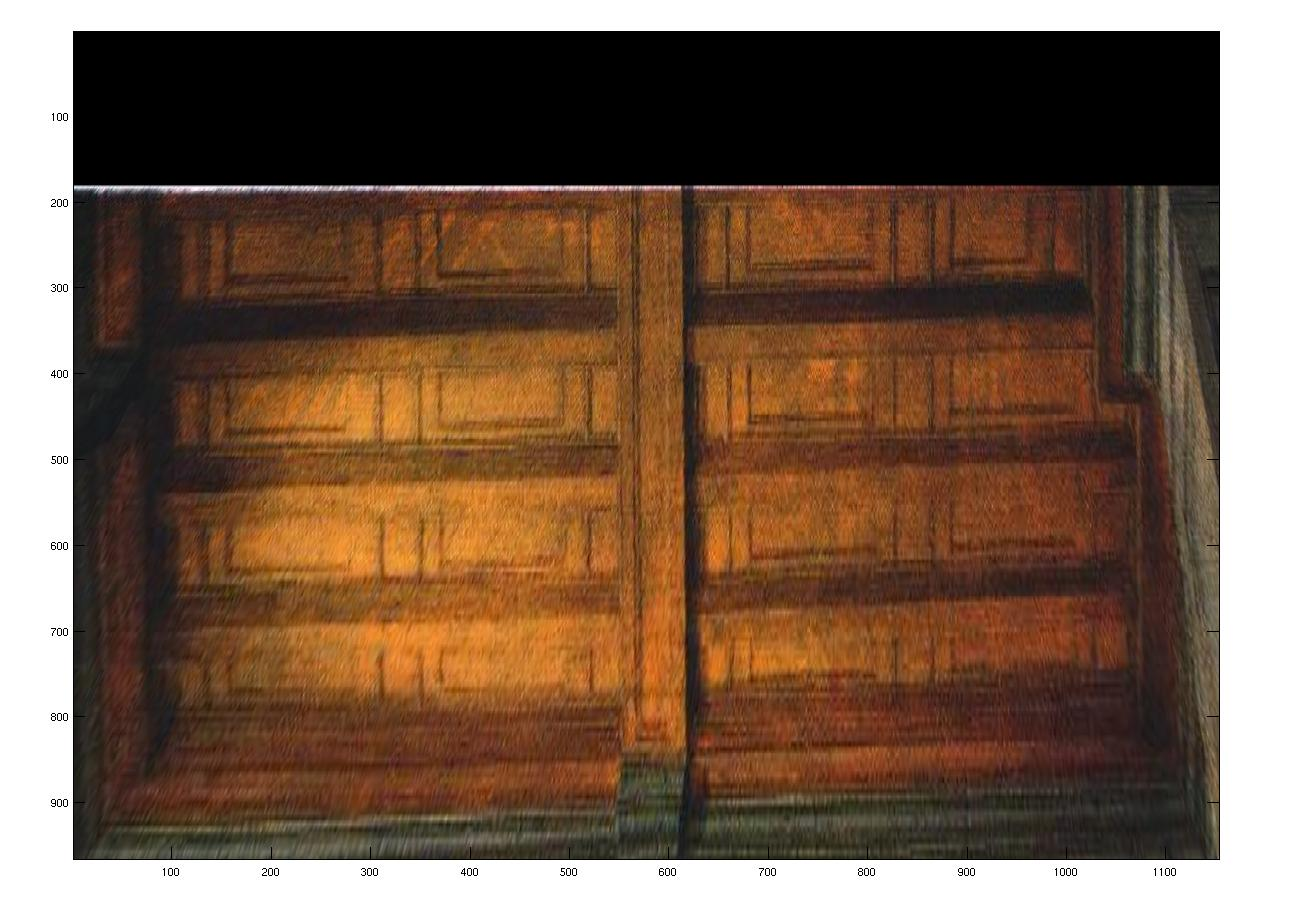
\includegraphics[width=0.5\linewidth]{./../img/ceiling.jpg}
    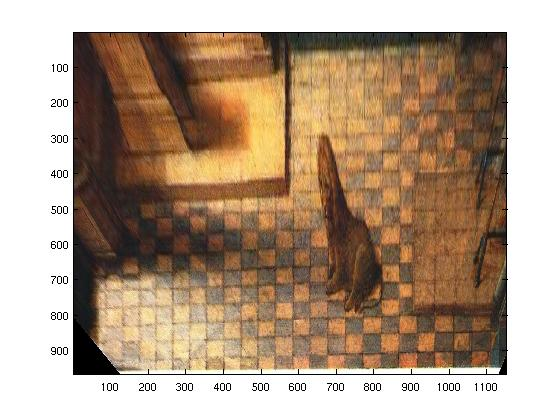
\includegraphics[width=0.5\linewidth]{./../img/floor.jpg}
    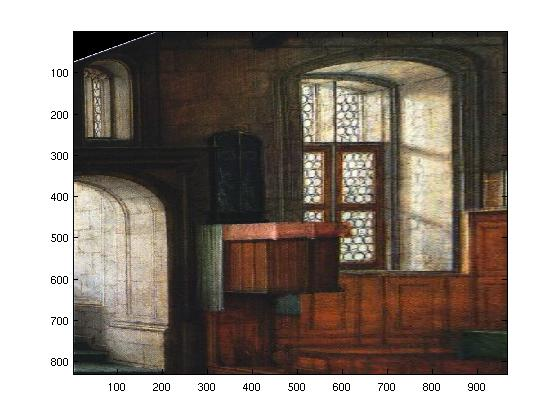
\includegraphics[width=0.5\linewidth]{./../img/left.jpg}
    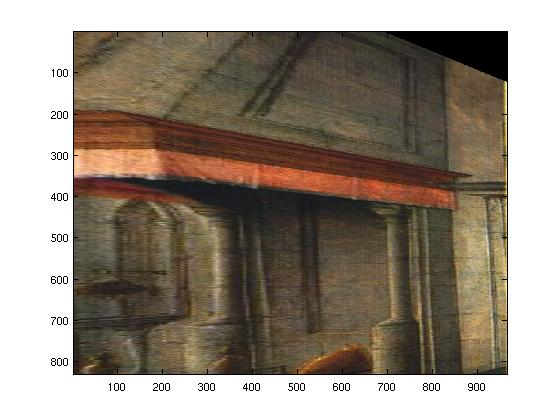
\includegraphics[width=0.5\linewidth]{./../img/right.jpg}
    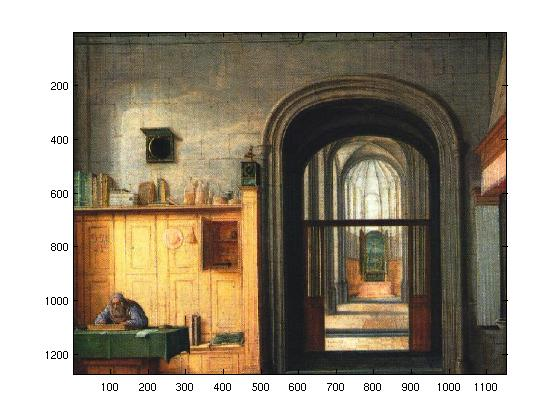
\includegraphics[width=0.5\linewidth]{./../img/back.jpg}

\item
    Views from sjerome.jpg:

    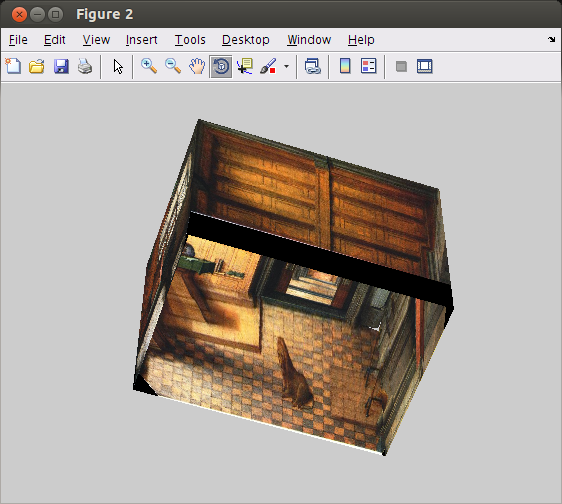
\includegraphics[width=0.5\linewidth]{./../img/sjerome_floor_ceiling.png}
    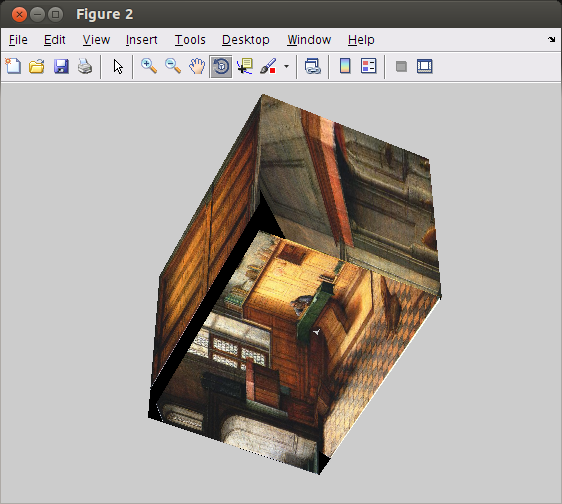
\includegraphics[width=0.5\linewidth]{./../img/sjerome_side_walls.png}

    Views from 320 Soda:

    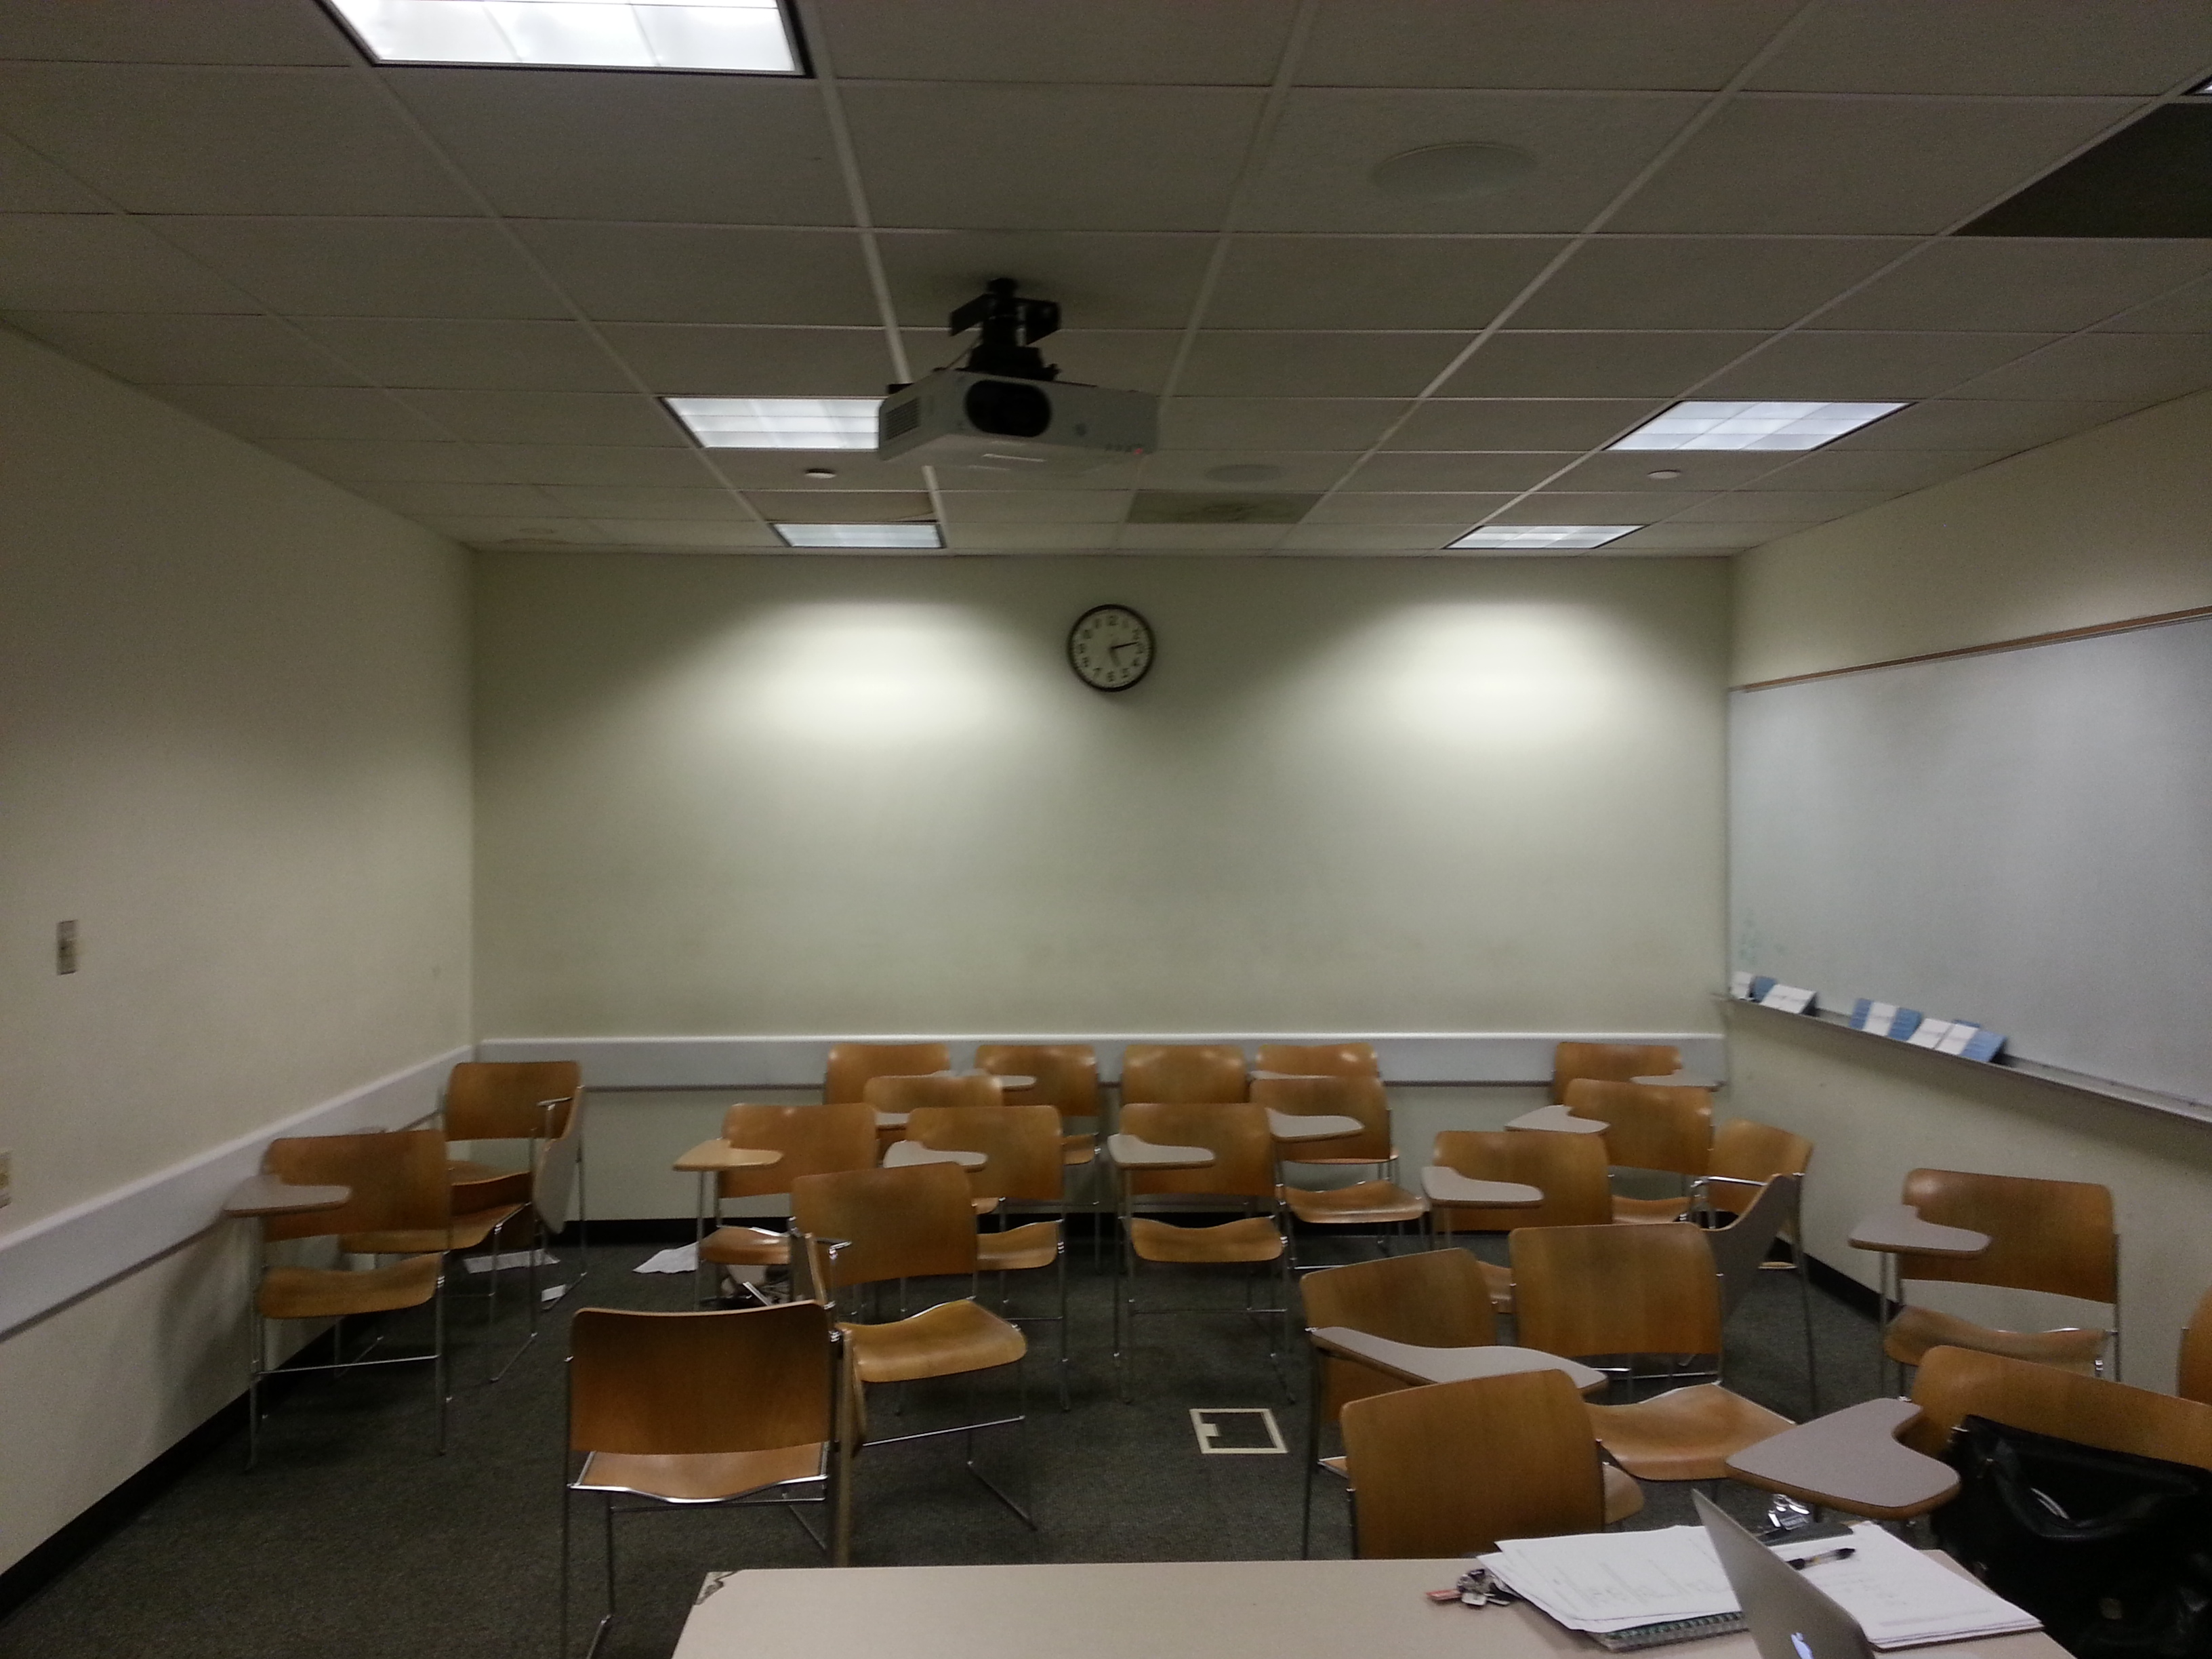
\includegraphics[width=0.5\linewidth]{./../img/TIP_1.jpg}
    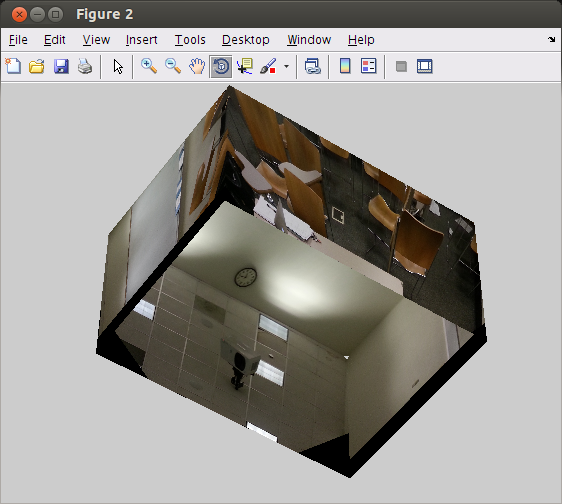
\includegraphics[width=0.5\linewidth]{./../img/TIP_1_ceiling.png}
    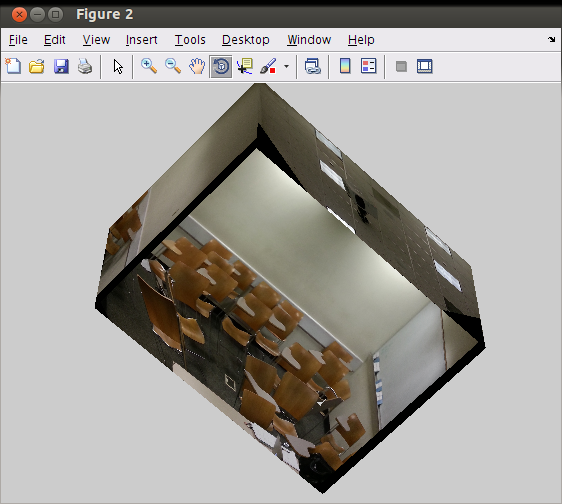
\includegraphics[width=0.5\linewidth]{./../img/TIP_1_whiteboard.png}

    Views from the Soda Etcheverry Breezeway:

    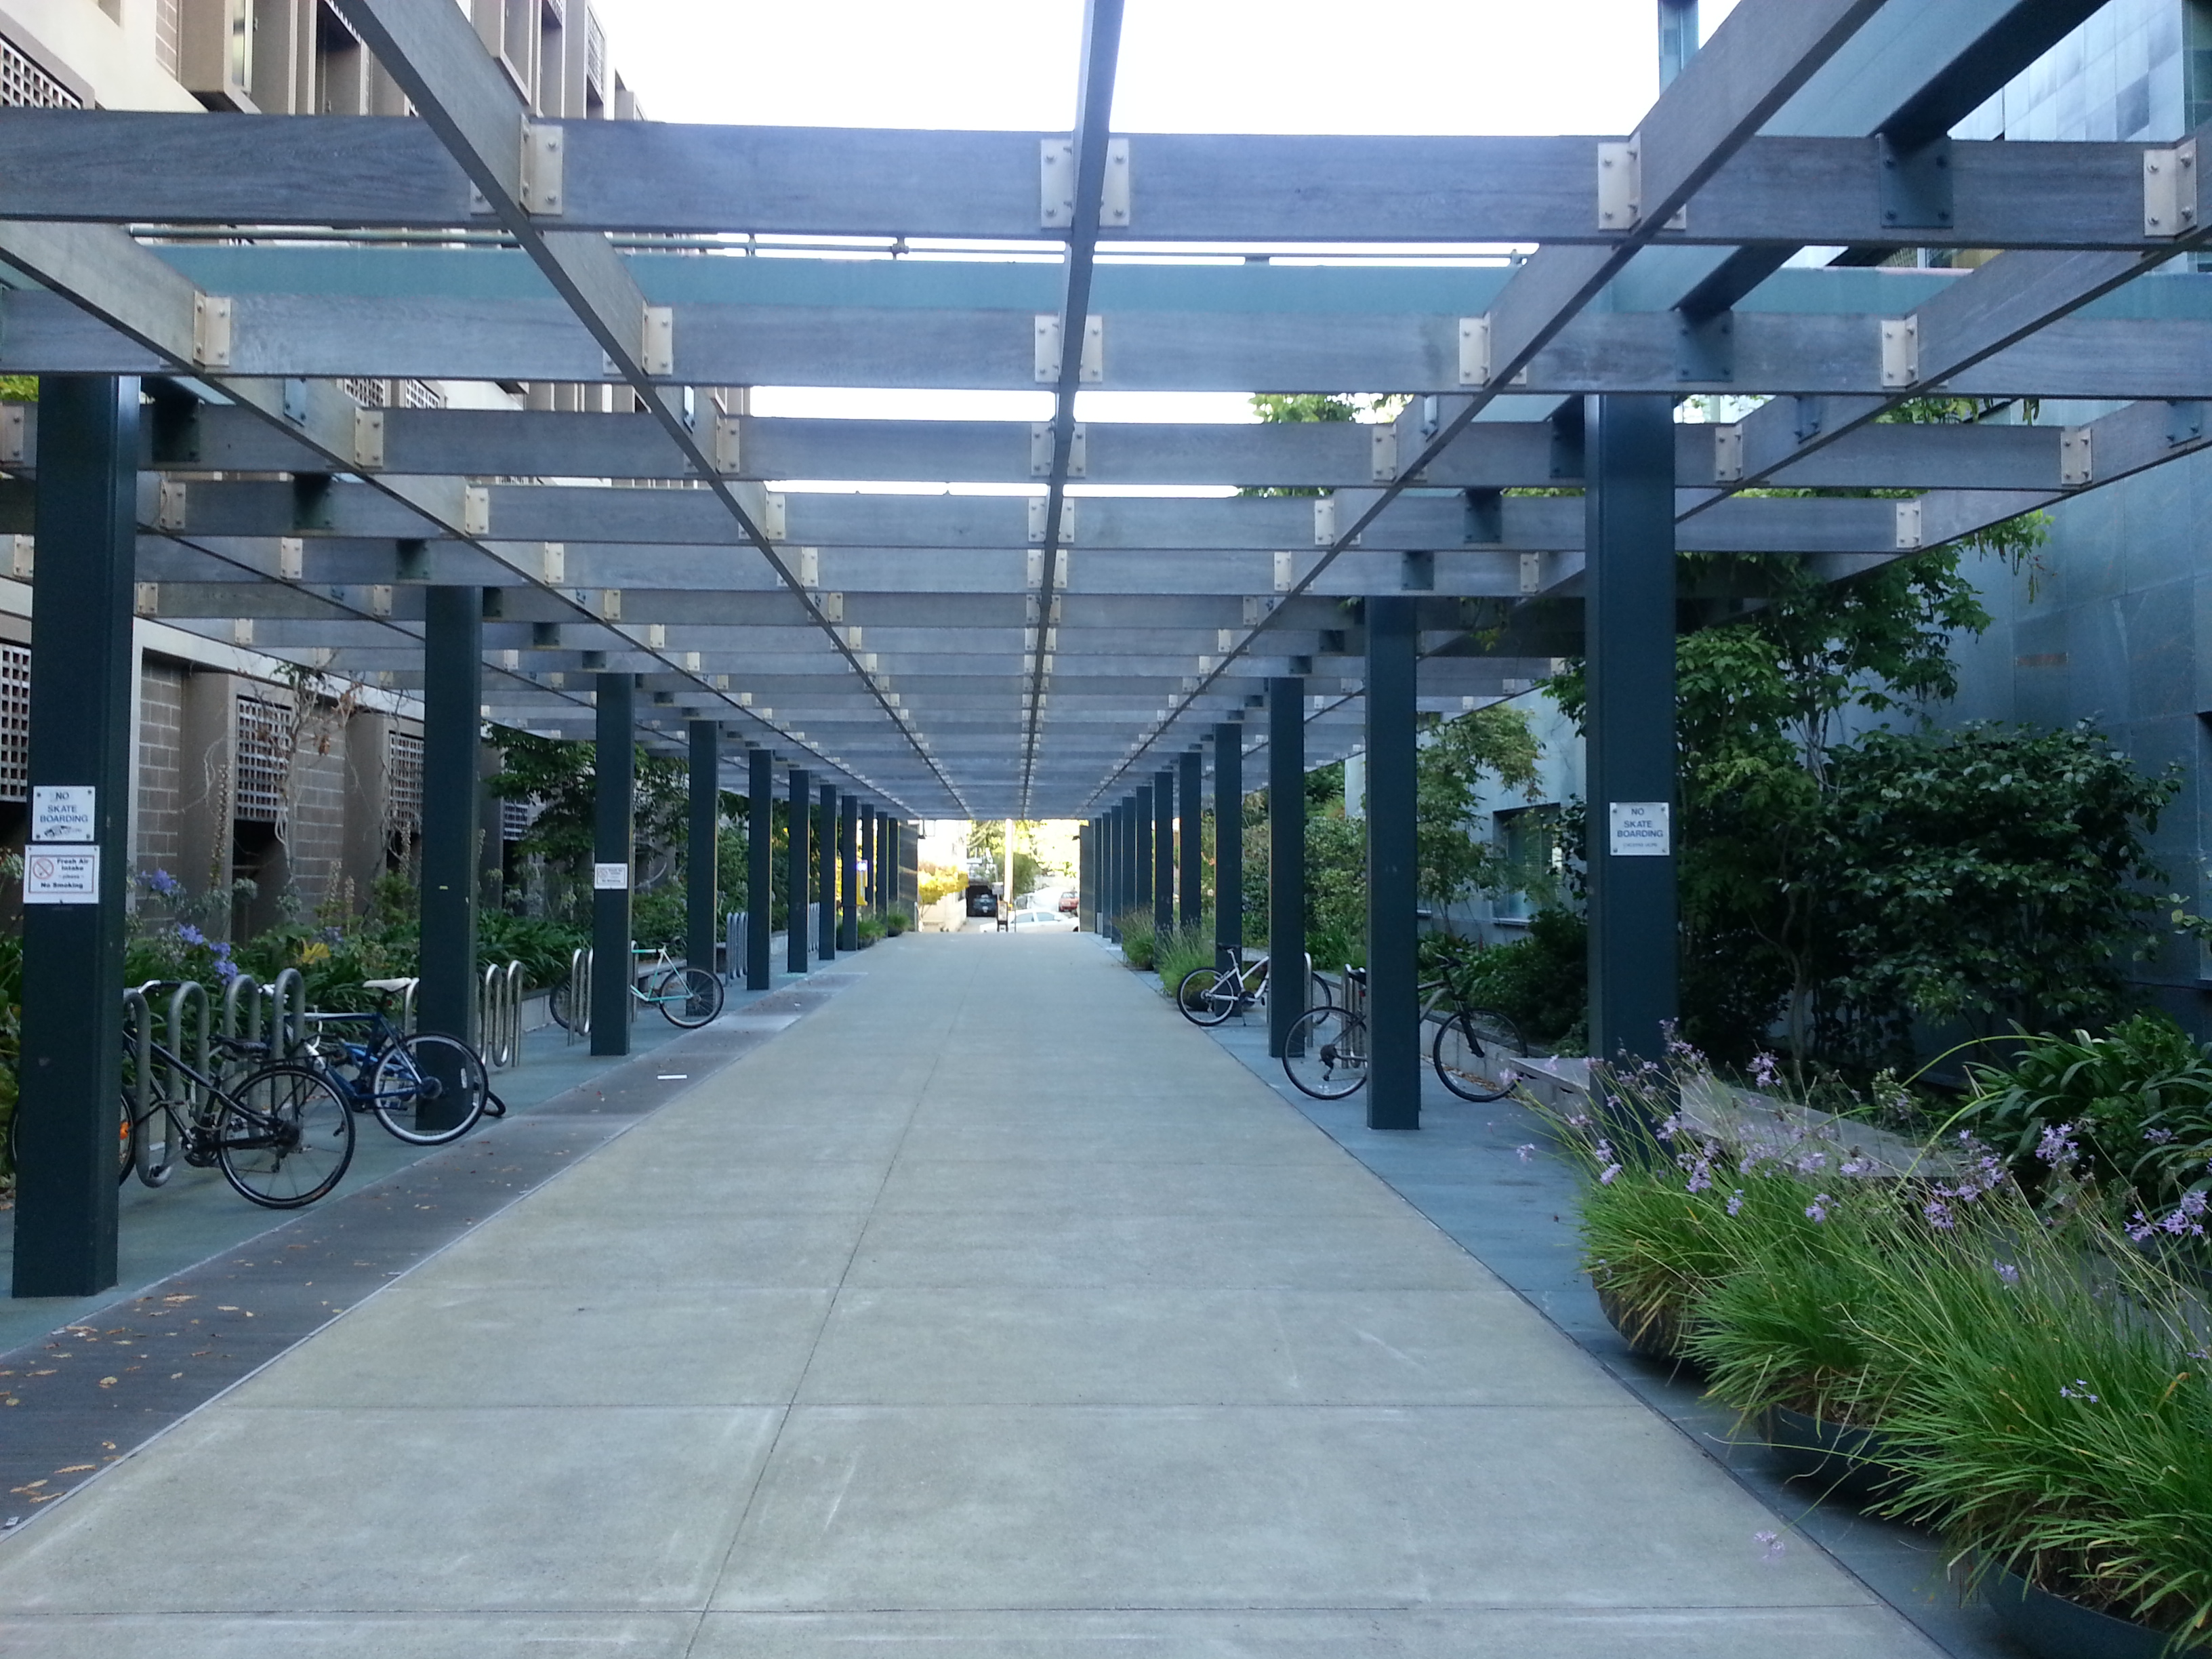
\includegraphics[width=0.5\linewidth]{./../img/TIP_2.jpg}
    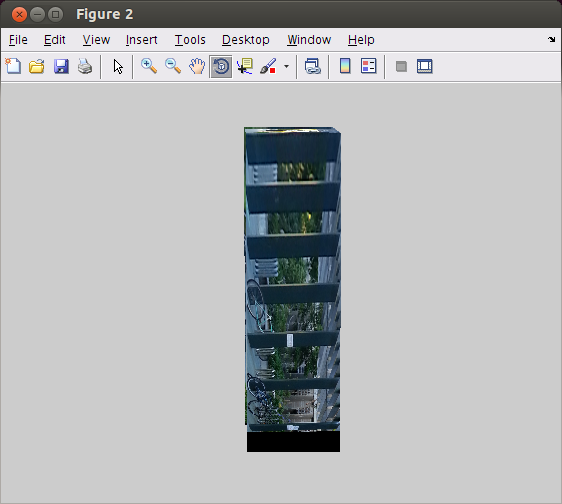
\includegraphics[width=0.5\linewidth]{./../img/TIP_2_columns.png}
    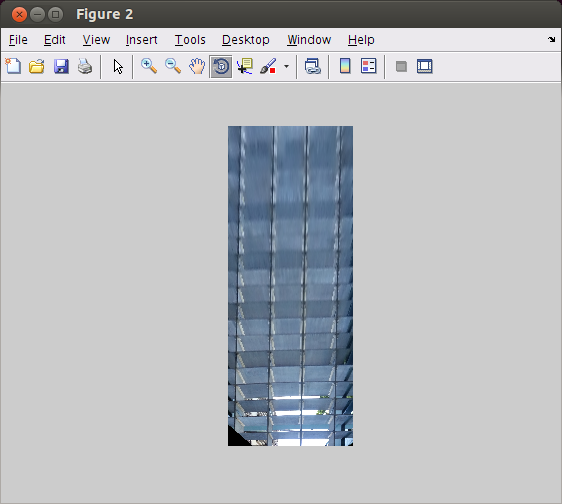
\includegraphics[width=0.5\linewidth]{./../img/TIP_2_rafters.png}
    % TODO bad
    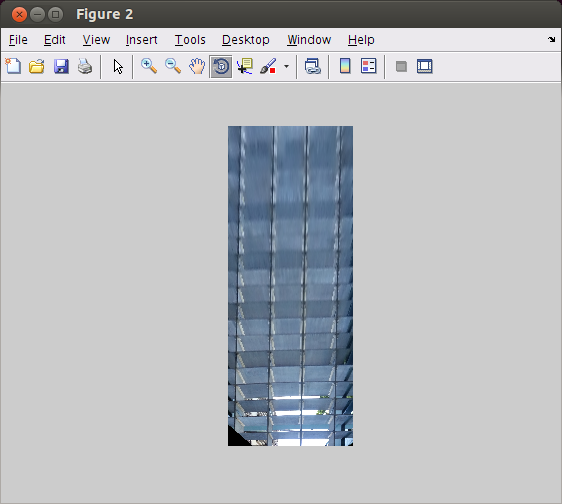
\includegraphics[width=0.5\linewidth]{./../img/TIP_2_rafters.png}

\end{enumerate}
\newpage

\section{Geometric Transformations}
\begin{enumerate}
\item
    We multiply the two reflection matrices and then use trigonometric
    sum/difference formulas.
    $$\begin{pmatrix}cos(2\beta)&sin(2\beta)\\sin(2\beta)&-cos(2\beta)\end{pmatrix}
    \begin{pmatrix}cos(2\alpha)&sin(2\alpha)\\sin(2\alpha)&-cos(2\alpha)\end{pmatrix} = $$

    $$\begin{pmatrix}cos(2\beta) cos(2\alpha) + sin(2\beta) sin(2\alpha) &
    sin(2\alpha) cos(2\beta) - cos(2\alpha) sin(2\beta) \\
    sin(2\beta) cos(2\alpha) - cos(2\beta) sin(2\alpha)&
    cos(2\alpha) cos(2\beta) + sin(2\alpha) sin(2\beta)\end{pmatrix} = $$

    $$\begin{pmatrix}cos(2(\beta-\alpha))&-sin(2(\beta-\alpha))\\
    sin(2(\beta-\alpha))&cos(2(\beta-\alpha))\end{pmatrix}$$
    
\item
    Consider a skew-symmetric matrix and its powers.
    $$\hat{s} = \begin{pmatrix}0&a&-b\\-a&0&c\\b&-c&0\end{pmatrix}$$
    $$\hat{s}^2 = \hat{s}^2$$
    $$\hat{s}^3 = (a^2 + b^2 + c^2)*-\hat{s}$$
    $$\hat{s}^4 = (a^2 + b^2 + c^2)*-\hat{s}^2$$
    $$\hat{s}^5 = (a^2 + b^2 + c^2)^2*\hat{s}$$
    $$...$$

    We know $||s|| = 1$, so we recognize a pattern.
    $$\hat{s} = \hat{s}$$
    $$\hat{s}^2 = \hat{s}^2$$
    $$\hat{s}^3 = -\hat{s}$$
    $$\hat{s}^4 = -\hat{s}^2$$
    $$...$$

    Now, we consider Roderigues' formula.
    $$R = e^{\phi\hat{s}}$$
    $$R = I + \phi\hat{s} + \frac{\phi^2\hat{s}^2}{2!} +
    \frac{\phi^3\hat{s}^3}{3!} + \frac{\phi^4\hat{s}^4}{4!}...$$

    Subbing in the powers of $\hat{s}$,
    $$R = I + \phi\hat{s} + \frac{\phi^2\hat{s}^2}{2!} -
    \frac{\phi^3\hat{s}}{3!} - \frac{\phi^4\hat{s}^2}{4!}...$$
    $$R = I + (\phi - \frac{\phi^3}{3!} + ...)\hat{s}
    + (\frac{\phi^2}{2!}  - \frac{\phi^4}{4!} + ...)\hat{s}^2$$
    $$R = I + sin(\phi)\hat{s} + (1 - cos(\phi))\hat{s^2}$$

\item
    The general form of a Euclidean planar transformation is $E$:
    $$\begin{pmatrix}cos\theta&-sin\theta&t_x\\sin\theta&cos\theta&t_y\\
    0&0&1\end{pmatrix}$$

    And a least squares problem is formulated as
    $$X\beta = y$$

    where $\beta$ consists of the unknown parameters.  Thus, we massage the
    problem into that form, saying $cos\theta$, $sin\theta$, $T_x$, and $T_y$
    are our parameters, so the problem is linear.
    $$\begin{pmatrix}x_1&-y_1&1&0\\y_1&x_1&0&1\\...\\x_n&-y_n&1&0\\y_n&x_n&0&1\end{pmatrix}
    \begin{pmatrix}cos\theta\\sin\theta\\T_x\\T_y\end{pmatrix} =
    \begin{pmatrix}x_1'\\y_1'\\...\\x_n'\\y_n'\end{pmatrix}$$

    Now we can plug in the given points to find an estimate for $E$.
    $$\beta = \begin{pmatrix}cos\theta\\sin\theta\\T_x\\T_y\end{pmatrix} = 
        (X^TX)^{-1}X^Ty$$

    For the given set of $u$ and $v$, we get:
    $$\beta = \begin{pmatrix}0\\-0.7857\\0\\0.75\end{pmatrix}$$

    Thus, our Euclidean planar transformation is:
    $$E = \begin{pmatrix}0&0.7857&0\\-0.7857&0&0.75\\0&0&1\end{pmatrix}$$

\item
\item
\end{enumerate}

\end{document}
